\documentclass[UTF-8]{ctexbeamer}
\usetheme{Boadilla}

\usepackage{listings}

\title{MeowRouter}
\subtitle{路由器的可扩展性及内卷}

\author{Grp.3 - 刘晓义\hspace{.2em} 娄晨耀 \hspace{.2em} 郑林楷 \hspace{.2em} 申奥}
\date{2019.12.25 - Merry Christmas}

\begin{document}
\begin{frame}
  \titlepage
\end{frame}
\begin{frame}
  \frametitle{Repository \& Contribution}

  \textbf{https://github.com/meow-chip}

  \begin{description}
    \item[MeowRouter] \textbf{数据平面 RTL} in Chisel3
    \item[MeowV64] \textbf{CPU RTL} in Chisel3
    \item[RouterSoftware] \textbf{控制平面固件} in Rust, asm, C++
    \item[MeowRouter\-top] \textbf{thinpad\_top} in admiration of 杰哥、橙橙和宇翔
  \end{description}

  \vspace{1em}

  \begin{description}
    \item[刘晓义] CPU 总体结构,数据平面流水设计,接口设计,Block Design 连连看
    \item[娄晨耀] 算法,转发表查找实现
    \item[郑林楷] 路由控制协议实现
    \item[申奥] CPU 执行单元,BPU
  \end{description}
\end{frame}
\begin{frame}
  \frametitle{Design Motivation}

  数据平面的核心工作:
  \begin{itemize}
    \item 解析、组装包
    \only<1>{\item 查找下一跳}
    \only<2->{\item \textbf{查找下一跳}}
    \item 填入 MAC
  \end{itemize}
  \vspace{1em}

  \pause
  \pause

  Currently(2019):

  \begin{itemize}
    \item 路由表可能很大 (813242 BGP prefixes @ 12-24\footnote{https://www.cidr-report.org/as2.0})
    \item 相比片上存储和 SRAM,大量的 DRAM 比较便宜,速度比较慢 (~20ns cmp. to ~5ns)
  \end{itemize}

  \pause
  \vspace{1em}

  核心目标:\textbf{减少访存}
\end{frame}
\begin{frame}
  \frametitle{Prior Arts}
  \begin{block}{Linux Netfilter Offload\footnote{https://www.kernel.org/doc/Documentation/networking/nf\_flowtable.txt}}
    \begin{center}
      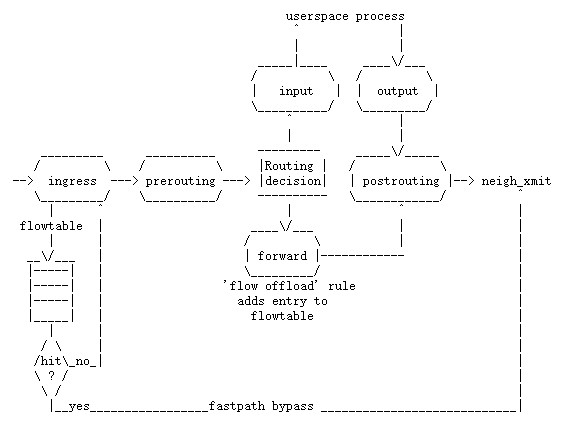
\includegraphics[width=0.6\textwidth]{assets/nf.jpg}
    \end{center}
  \end{block}
\end{frame}
\begin{frame}
  \frametitle{Prior Arts}
  \begin{block}{Luleå algorithm}
    Trie Tree, 为通用计算硬件设计(General-purpose CPU + Cache)

    单次查找 \textasciitilde 8 次访存

    有针对快速更新的优化
  \end{block}
  \pause
  \begin{block}{CuckooSwitch}
    使用 Cuckoo Hashtable 查询交换规则
  \end{block}
\end{frame}

\begin{frame}
  \frametitle{Algorithm}

  转发表由 /32 -> /32 的转发规则构成,使用软件计算后填充到硬件内

  \begin{itemize}
    \item 存储可以使用哈希表
    \item 硬件可以通过直接按位比较处理
    \item 方便添加额外信息: NAT etc.
  \end{itemize}

  \pause
  \vspace{1em}

  如何修改?

  \pause
  
  \vspace{1em}

  哈希表的设计?
  \begin{description}
    \item[Identity] 需要 $2^{32} \times 32\text{bit}$ = 16GB RAM,保证单次访存
    \item[Open addressing] 访存数量不定,需要用利用率换平均访存速度: Swisstable
    \item[Chaining] 硬件没法实现
  \end{description}
\end{frame}
\begin{frame}
  \frametitle{Cuckoo Hashtable}

  \begin{itemize}
    \item 哈希函数得到两个值
    \item 每个 Key 对应两个 Index,如果插入的时候两行都满了,可以通过将某一位置的内容移动到它对应的另一行中
    \item 查询保证两次访存,硬件实现简单
    \item 可以达到 95\% 的利用率
    \item 插入逻辑较复杂,访存可能比较多: CPU Cache
  \end{itemize}
\end{frame}

\begin{frame}
  \frametitle{Memory Access}

  使用标准总线: \textbf{AXI}
  
  \pause

  \vspace{1em}
  Pros:

  \begin{itemize}
    \item 有很多的 IP 可以用: UART, BRAM, EMC, ...
    \item 扩展性高:Interconnect 上 Master 和 Slave 数量不定,可以级联
  \end{itemize}

  \vspace{1em}
  Cons:
  \begin{itemize}
    \item 延迟高: At least 10 Cycles
    \item 占用片上面积很大: tot. 10K LUT
  \end{itemize}
\end{frame}

\begin{frame}
  \frametitle{Overall picture}

  \begin{center}
    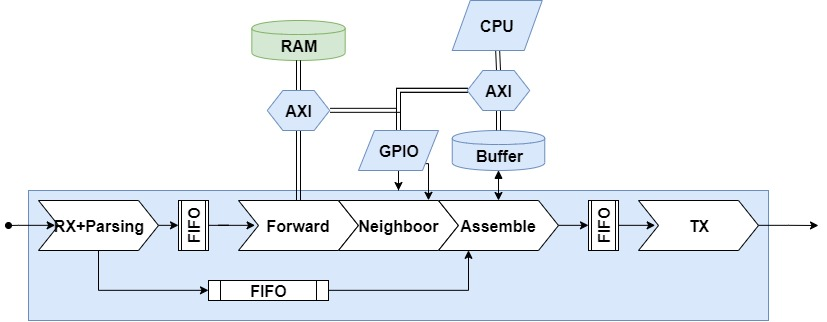
\includegraphics[width=0.95\textwidth]{assets/overall-pic.jpg}
  \end{center}
\end{frame}

\begin{frame}
  \frametitle{Optimization}

  为了保证数据平面的处理速度最大化,进行了以下优化:
  \begin{itemize}
    \item 采用两级 AXI Interconnect,第二级连接 EMC,使用数据平面的 125M 时钟
    \item 发送读取请求时,采用 Request Interleaving: 减小 Interconnect 带来的延迟
    \item 移除所有空转的自动机状态
    \item 增大 CPU 的 rx/tx buffer,减少短期 Burst 带来的丢包,让一轮能够计算得到的转发规则更多
  \end{itemize}
\end{frame}

\begin{frame}
  \frametitle{Performance}
  \begin{description}
    \item[单口单工] \textasciitilde 94 Mbps
    \item[单口双工] \textasciitilde 187 Mbps
    \item[双口双工] \textasciitilde 330 Mbps
    \item[小包] \textasciitilde 148kpps
  \end{description}
\end{frame}

\begin{frame}
  \frametitle{CPU brief intro.}

  \begin{itemize}
    \item 70M, 默认配置使用 \textasciitilde 50K LUT
    \pause
    \item 64bit RISC-V, 实现 ISA 为 \textbf{RV64IMAC -Zifencei -Zicsr}
    \begin{description}
      \item[I] 整数指令集
      \item[M] 乘除法
      \item[A] Atomic Primitives
      \item[C] 压缩指令集
      \item[-Zifencei] FENCE.I
      \item[-Zicsr] CSR 及指令
    \end{description}
    \pause
    \item 流水线: \textbf{多发射 + 预测执行(BHT + RAS) + 乱序执行(Tomasulo)}
    \begin{itemize}
      \item ALU 1 + Branch + CSR + Bypass
      \item ALU 2 + Mul + Div
      \item LSBuf + LSU
    \end{itemize}
    \pause
    \item Cache: \textbf{L1 Instr/Data, L2 + MSI Directory, 支持多核}
    \item 可配置
  \end{itemize}
\end{frame}

\begin{frame}
  \frametitle{Firmware}

  \begin{itemize}
    \item 汇编编写固件入口,Trap Vector 入口,初始化栈指针,传入 mhartid
    \item Rust 编写 Firmware 的转发表项计算、填入,ARP 表项填入,发包、收包逻辑,HAL 后端
    \item C 编写 RIP 协议部分
  \end{itemize}

  Linker Script 将 .text 和 .rodata 放到 Flash 中,将 .data 放到 SRAM 中

  不使用 BSS 段: 懒得清空
\end{frame}

\begin{frame}
  \frametitle{RIP}

  基础是 Router-Lab,方便脱离其他部分调试

  实现了 Split horizon, Poisoned reverse
  
  \pause
  
  \vspace{1em}

  尝试解决 RIP 处理速度慢的问题:

  根据 UDP Checksum 随机丢包

  \pause
  
  \vspace{1em}

  由于和 RIP 无关的固件问题,目前最多存储大约 1500 条表项,之后会栈溢出

\end{frame}

\begin{frame}
  \frametitle{Tools}

  \textbf{Chisel3}

  用 Scala 的 DSL 做 HDL,更强的编译期检查,可配置性

  https://github.com/freechipsproject/chisel3

  \pause

  \vspace{1em}

  \textbf{Block Design}

  Vivado 提供的可视化编程(?)工具

  连连看,方便配置 IP
\end{frame}

\begin{frame}
  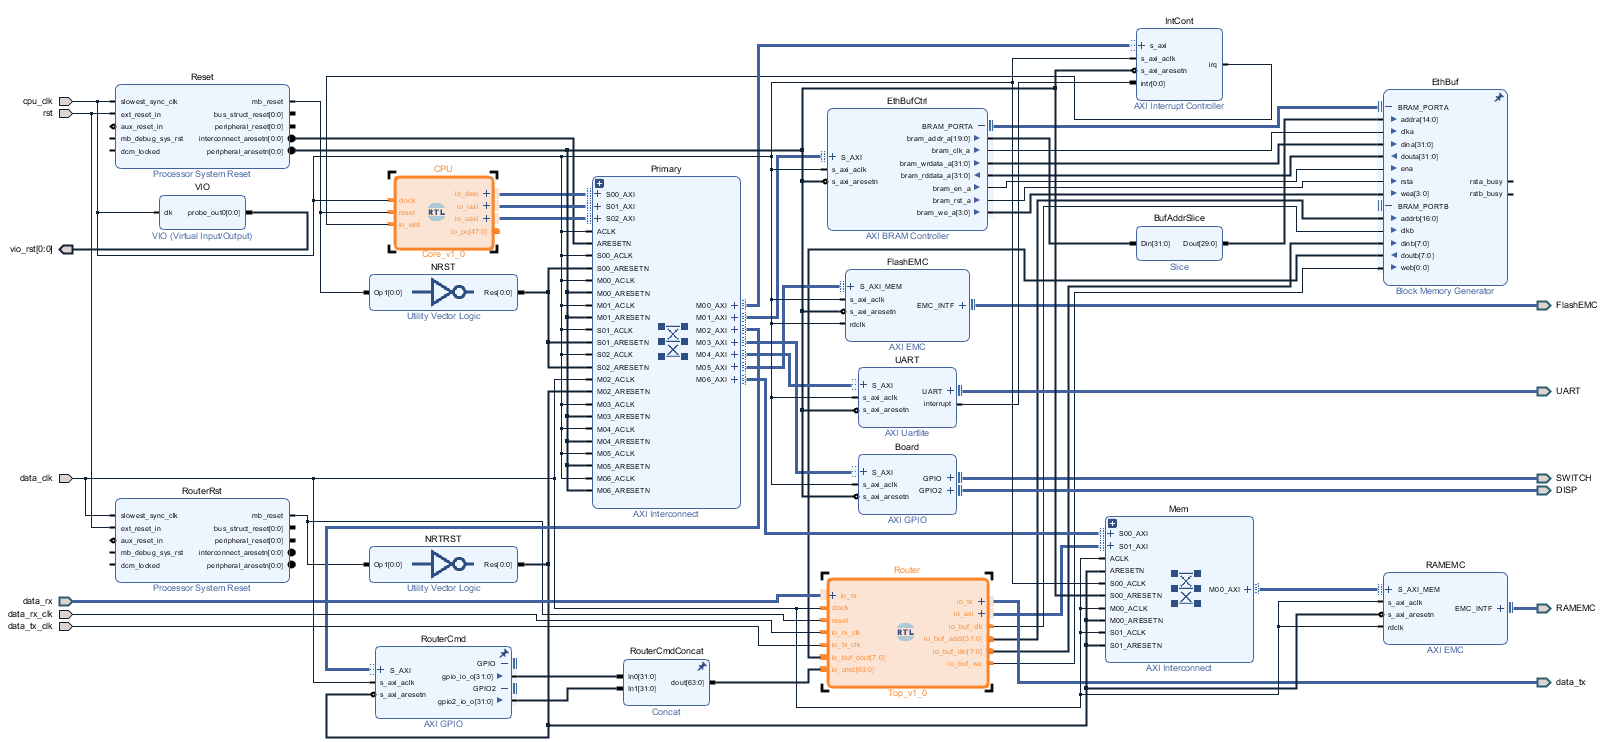
\includegraphics[width=\textwidth]{assets/bd.png}
\end{frame}

\begin{frame}
  \frametitle{Thanks!}

  \begin{center}
    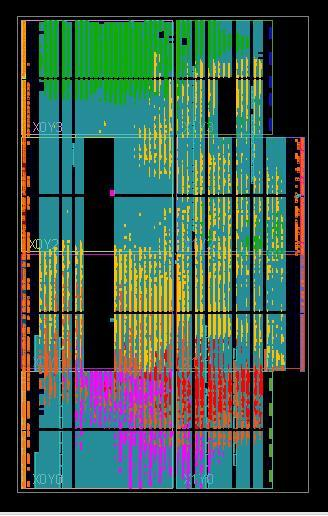
\includegraphics[height=0.7\textheight]{assets/board.jpg}
  \end{center}
\end{frame}
\end{document}
